\documentclass[../main.tex]{subfiles}


\begin{document}

\chapter{}
\label{cha:cha_1}


\section{}
You are given the following differential equation with the initial condition, v(t = 0) = 0,
\bigbreak
\label{sec:sec_1_1}
$\dfrac{d v}{d t}=g-\dfrac{c_{d}}{m} v^{2}$

	\bigbreak
Multiply both sides by $m / c_{d}$
	\bigbreak
$\dfrac{m}{c_{d}} \dfrac{d v}{d t}=\dfrac{m}{C_{d}} g-v^{2}$
	\bigbreak
Define $a=\sqrt{m g / c_{d}}$
	\bigbreak
$\dfrac{m}{c_{d}} \dfrac{d v}{d t}=a^{2}-v^{2}$
	\bigbreak
Integrate by separation of variables,
	\bigbreak
$\int \dfrac{d v}{a^{2}-v^{2}}=\int \dfrac{c_{d}}{m} d t$
	\bigbreak
A table of integrals can be consulted to find that
	\bigbreak
$\int \dfrac{d x}{a^{2}-x^{2}}=\dfrac{1}{a} \tanh ^{-1} \dfrac{x}{a}$
	\bigbreak
Therefore, the integration yields
	\bigbreak
$\dfrac{1}{a} \tanh ^{-1} \dfrac{v}{a}=\dfrac{C_{d}}{m} t+C$
	\bigbreak
If $v=0$ at $t=0$, then because $\tanh ^{-1}(0)=0$, the constant of integration $C=0$ and the solution is
	\bigbreak
$\dfrac{1}{a} \tanh ^{-1} \dfrac{v}{a}=\dfrac{c_{d}}{m} t$
	\bigbreak
This result can then be rearranged to yield
	\bigbreak
$v=\sqrt{\dfrac{g m}{c_{d}}} \tanh \left(\sqrt{\dfrac{g c_{d}}{m}} t\right)$
	\bigbreak


\section{}
This is a transient computation. For the period from ending June 1 :
\bigbreak
\label{sec:sec_1_2}
\pagebreak
Balance = Previous Balance + Deposits - Withdrawals
	\bigbreak
Balance =1512.33+220.13-327.26=1405.20
	\bigbreak
The balances for the remainder of the periods can be computed in a similar fashion as 
tabulated below:
\bigbreak

	\begin{tabular}{|c|c|c|c|c|}
		\hline
		Date & Deposit & Withdrawal & Balance \\ \hline
		1-May &  &  & $\$ 1512.33$ \\ \hline
		 & $\$ 220.13$ & $\$ 327.26$ &  \\ \hline
		1-Jun &  &  & $\$ 1405.20$ \\ \hline
		 & $\$ 216.80$ & $\$ 378.61$ &  \\ \hline
		1-Jul &  &  & $\$ 1243.39$ \\ \hline
		 & $\$ 350.25$ & $\$ 106.80$ &  \\ \hline
		1-Aug &  &  & $\$ 1586.84$ \\ \hline
		 & $\$ 127.31$ & $\$ 450.61$ &  \\ \hline
		1-Sep &  &  & $\$ 1363.54$ \\ \hline
	\end{tabular}	
	\bigbreak


\section{ }
At t = 12 s, the analytical solution is 50.6175 (Example 1.1). The numerical results are:
\bigbreak
	\begin{tabular}{|c|c|c|}
		\hline
		step & $\mathrm{v}(12)$ & absolute relative error \\
		\hline
		2 & $51.6008$ & $1.94 \%$ \\
		\hline
		1 & $51.2008$ & $1.15 \%$ \\
		\hline
		$0.5$ & $50.9259$ & $0.61 \%$ \\
		\hline
	\end{tabular}
	\bigbreak
where the relative error is calculated with
	\bigbreak
absolute relative error $=\left|\dfrac{\text { analytical }-\text { numerical }}{\text { analytical }}\right| \times 100 \%$
	\bigbreak
The error versus step size can be plotted as
	\bigbreak
	\begin{figure}[H]
		\hspace{1cm}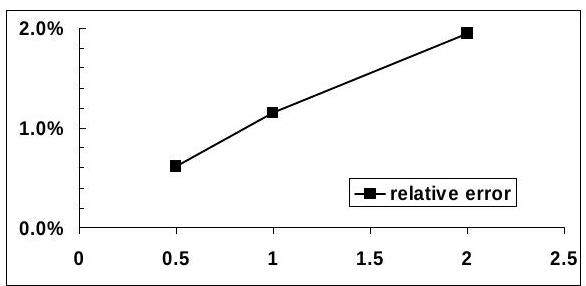
\includegraphics[width=0.5\linewidth]{fig_1_1}
		\label{fig:fig_1_1}
	\end{figure}
	\bigbreak
Thus, halving the step size approximately halves the error.
	\bigbreak

\section{ }

\begin{enumerate}[label=\bfseries(\alph*)]

\item The force balance is
\bigbreak
$\dfrac{d v}{d t}=g-\dfrac{c^{\prime}}{m} v$
\bigbreak

Applying Laplace transforms,
\bigbreak
$s V-v(0)=\dfrac{g}{s}-\dfrac{c^{\prime}}{m} V$
\bigbreak
Solve for
\bigbreak


\begin{equation} \hspace{-12cm}V=\dfrac{g}{s\left(s+c^{\prime} / m\right)}+\dfrac{v(0)}{s+c^{\prime} / m}\tag{1}\end{equation} 


\bigbreak
The first term to the right of the equal sign can be evaluated by a partial dfraction expansion,
\bigbreak


\begin{equation}\hspace{-12cm}\dfrac{g}{s\left(s+c^{\prime} / m\right)}=\dfrac{A}{s}+\dfrac{B}{s+c^{\prime} / m} \tag{2}\end{equation} 
\bigbreak
$\dfrac{g}{s\left(s+c^{\prime} / m\right)}=\dfrac{A\left(s+c^{\prime} / m\right)+B s}{s\left(s+c^{\prime} / m\right)}$


\bigbreak
Equating like terms in the numerators yields
\bigbreak
$
\begin{aligned}
&A+B=0 \\
&g=\dfrac{c^{\prime}}{m} A
\end{aligned}
$
\bigbreak
Therefore,
\bigbreak
$A=\dfrac{m g}{c^{\prime}} \quad B=-\dfrac{m g}{c^{\prime}}$
\bigbreak
These results can be substituted into Eq. (2), and the result can be substituted back into Eq.
\newline
(1) to give
\bigbreak

$V=\dfrac{m g / c^{\prime}}{s}-\dfrac{m g / c^{\prime}}{s+c^{\prime} / m}+\dfrac{v(0)}{s+c^{\prime} / m}$
\bigbreak
Applying inverse Laplace transforms yields
\bigbreak
$v=\dfrac{m g}{c^{\prime}}-\dfrac{m g}{c^{\prime}} e^{-\left(c^{\prime} / m\right) t}+v(0) e^{-\left(c^{\prime} / m\right) t}$
\bigbreak
or
\bigbreak
$v=v(0) e^{-\left(c^{\prime} / m\right) t}+\dfrac{m g}{c^{\prime}}\left(1-e^{-\left(c^{\prime} / m\right) t}\right)$
\bigbreak
where the first term to the right of the equal sign is the general solution and the second is the particular solution. For our case, v(0)=0, so the final solution is
\bigbreak
\fbox {$v=\dfrac{m g}{c^{\prime}}\left(1-e^{-\left(c^{\prime} / m\right) t}\right)$}
\bigbreak
\item The numerical solution can be implemented as
\bigbreak
$
\begin{aligned}
&v(2)=0+\left[9.81-\dfrac{12.5}{68.1}(0)\right] 2=19.62 \\
&v(4)=19.62+\left[9.81-\dfrac{12.5}{68.1}(19.62)\right] 2=6.2087
\end{aligned}
$
\bigbreak
The computation can be continued and the results summarized and plotted as:
\bigbreak

\begin{tabular}{ccc}
	t&v&dv/dt\\
	0 & 0 & 9.81\\
	2 & 19.6200 & 6.2087\\
	4 & 32.0374 & 3.9294 \\
	 6 & 39.8962 & 2.4869\\
	8 & 44.8700 & 1.5739\\
	10 & 48.0179 & 0.9961\\
	12 & 50.0102 & 0.6304\\
	\end{tabular}
	\bigbreak
\begin{figure}[H]
		\hspace*{1cm}\fbox{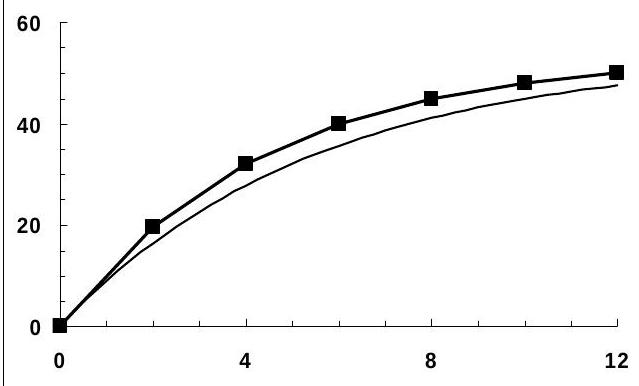
\includegraphics[width=0.5\linewidth]{fig_1_2}}
		\label{fig:fig_1_2}
	\end{figure}
	\bigbreak
Note that the analytical solution is included on the plot for comparison.
\bigbreak
\end{enumerate}
\section{ }
\begin{enumerate}[label=\bfseries(\alph*)]
\item The first two steps are
\bigbreak
$
\begin{aligned}
&c(0.1)=10-0.2(10) 0.1=9.8 \mathrm{~Bq} / \mathrm{L} \\
&c(0.2)=9.8-0.2(9.8) 0.1=9.604 \mathrm{~Bq} / \mathrm{L}
\end{aligned}
$
\bigbreak
The process can be continued to yield
\bigbreak

\begin{tabular}{crr}
\Xhline{1.5pt}
$t$ & \multicolumn{1}{c}{$c$} & \multicolumn{1}{c}{$d c / d t$} \\
\hline
0 & $10.0000$ & $-2.0000$ \\
$0.1$ & $9.8000$ & $-1.9600$ \\
$0.2$ & $9.6040$ & $-1.9208$ \\
$0.3$ & $9.4119$ & $-1.8824$ \\
$0.4$ & $9.2237$ & $-1.8447$ \\
$0.5$ & $9.0392$ & $-1.8078$ \\
$0.6$ & $8.8584$ & $-1.7717$ \\
$0.7$ & $8.6813$ & $-1.7363$ \\
$0.8$ & $8.5076$ & $-1.7015$ \\
$0.9$ & $8.3375$ & $-1.6675$ \\
1 & $8.1707$ & $-1.6341$ \\
\Xhline{1.5pt}
\end{tabular}
\bigbreak

\item The results when plotted on a semi-log plot yields a straight line
\bigbreak

\begin{figure}[H]
		\hspace*{1cm}\fbox{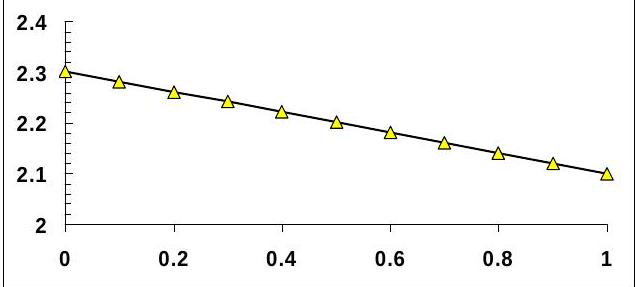
\includegraphics[width=0.5\linewidth]{fig_1_3}}
		\label{fig:fig_1_3}
	\end{figure}
	\bigbreak

The slope of this line can be estimated as
\bigbreak
$\dfrac{\ln (8.1707)-\ln (10)}{1}=-0.20203$
\bigbreak
Thus, the slope is approximately equal to the negative of the decay rate.
\bigbreak


\section{ }
The first two steps yield
\bigbreak
$
\begin{aligned}
&y(0.5)=0+\left[3 \dfrac{400}{1200} \sin ^{2}(0)-\dfrac{400}{1200}\right] 0.5=0+[0-0.33333] 0.5=-0.16667 \\
&y(1)=-0.16667+\left[\sin ^{2}(0.5)-0.333333\right] 0.5=-0.21841
\end{aligned}
$
\bigbreak
The process can be continued to give
\bigbreak

\begin{tabular}{|c|c|}
\hline
$\mathrm{t}$ & $\mathrm{y}$ \\
\hline
0 & 0 \\
\hline
$0.5$ & $-0.16667$ \\
\hline
1 & $-0.21841$ \\
\hline
$1.5$ & $-0.03104$ \\
\hline
2 & $0.299793$ \\
\hline
$2.5$ & $0.546537$ \\
\hline
3 & $0.558955$ \\
\hline
$3.5$ & $0.402245$ \\
\hline
4 & $0.297103$ \\
\hline
$4.5$ & $0.416811$ \\
\hline
5 & $0.727927$ \\
\hline
\end{tabular}
\bigbreak

\begin{figure}[H]
		\hspace*{1cm}{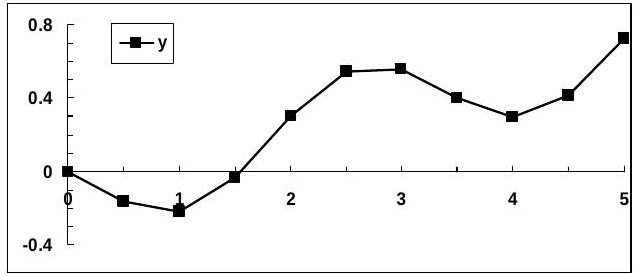
\includegraphics[width=0.5\linewidth]{fig_1_4}}
		\label{fig:fig_1_4}
	\end{figure}
	\bigbreak

\section{ }
$v(t)=\dfrac{g m}{c}\left(1-e^{-\left(\dfrac{c}{m}\right) t}\right)$

jumper \#1: $v(t)=\dfrac{9.8(68.1)}{12.5}\left(1-e^{-\left(\dfrac{12.5}{68.1}\right)}\right)=44.87 \mathrm{~m} / \mathrm{s}$

jumper \#2: $44.87=\dfrac{9.8(75)}{14}\left(1-e^{-\left(\dfrac{14}{75}\right) t}\right)$

$44.87=52.5-52.5 e^{-0.18666 t}$
\bigbreak
$0.14533=e^{-0.18666 t}$\newline
$\ln 0.14533=\ln e^{-0.18666 t}$
\bigbreak
$\bold{ t=10.33 \mathrm\bold\hspace*{0.1cm}{sec}}$
\bigbreak

\section{ }
$ Q_{\text {in }}=Q_{\text {out }}$
\bigbreak
$Q_{1}=Q_{2}+Q_{3}$
\bigbreak
$30=20+v A_{3}$
\bigbreak
$10=5\hspace*{0.1cm} A_{3}$
\bigbreak
$A_{3}=2 \mathrm{~m}^{2}$
\bigbreak

\section{ }

$\sum M_{i n}-\sum M_{\text {out }}=0$
\bigbreak
$[1000+1200+\mathrm{MP}+50]-[400+200+1400+200+350]=0$
\bigbreak
Metabolic production = 300 grams

\section{ }
$
\begin{aligned}
\sum \%  \text { body weight }= 60
\end{aligned}
$
\bigbreak
4.5 + 4.5 + 12 + 4.5 + 1.5 + IW = 60
\bigbreak
\textbf{\% Intracellular water body weight = 33 \%}
\bigbreak

4.5 + 4.5 + 12 + 4.5 + 1.5 + IW = 60
\bigbreak
$
\begin{aligned}
&\sum \% \text { body water } = 100 \\ 
\end{aligned}
$
\bigbreak
7.5 + 7.5 + 20 + 7.5 + 55 + TW = 100

\bigbreak
\textbf{\% Transcellular water of body water = 2.5 \%}


\end{enumerate}
\end{document}

